\documentclass[fleqn]{jbook}
\usepackage{physpub}

\begin{document}

\begin{question}{専攻 問題2}{}

$z$方向に一様で断面の形が一定な中空の導体管内をz方向に伝播する電磁波を
考える(図1)。真空の誘電率を$\varepsilon_{0}$、真空の透磁率を$\mu_{0}$と
する時、以下の設問に答えよ。

\begin{subquestions}
\SubQuestion
  ある境界条件のもとでMaxwell方程式に従う電場、磁場をそれぞれ
%
  \begin{equation}
    \vec{E}=\vec{E_{0}}(x,y) \exp \{ i(kz-\omega t) \} \hspace{15mm}%
    \vec{H}= \vec{H_{0}}(x,y) \exp \{ i(kz-\omega t) \} \eqname{1}
  \end{equation}
%
  とし
%
  \[ \vec{E_{0}}=( E_{x},E_{y},E_{z} ) \hspace{15mm}%
     \vec{H_{0}}=( H_{x},H_{y},H_{z} ) \]
%
  と置く時、$E_{x},E_{y},H_{x},H_{y}$を
  $\ds\frac{\partial E_{z}}{\partial x},
  \ds\frac{\partial E_{z}}{\partial y},
  \ds\frac{\partial H_{z}}{\partial x},
  \ds\frac{\partial H_{z}}{\partial y}$で表せ。

\SubQuestion
  $E_{z},H_{z}$がそれぞれ満たす二階偏微分方程式を求めよ。又、このよう
  な導体管内を伝播する電磁波は、TM波とTE波に分けて考えることができる。
  その理由を述べよ。 但し、TM波とは進行方向の磁場成分が0であるような
  電磁波であり、TE波とは進行方向の電場成分が0であるような電磁波である。

\SubQuestion
  図2のように、断面が長方形$(a \!\! > \!\! b)$の時、$\omega$と$k$との
  関係を求めよ。又、位相速度を$v_{p}(=\omega / k)$、群速度を
  $v_{g}(=\partial \omega / \partial k)$とする時
%
  \[ v_{p} \cdot v_{g} = c^{2} \]
%
  である事を示せ。但し、
  $c^{2}=\ds\frac{1}{\varepsilon_{0} \mu_{0}}$である。

\SubQuestion
  前問で最小の$\omega$を与える電場、磁場を求めよ。

\SubQuestion
  電磁波の進行方向に一定の間隔$L$で同じ形の導体板を取り付けた
  (図3)。この時の$\omega$と$k$の関係について議論せよ。\\
  ヒント:$E(z)$が解である時、$E(z+L)$も解である事を使え。

\end{subquestions}

--------------------------------------------------------------------------------------------------------------\\

\begin{minipage}{60mm}
(参考)Maxwell方程式は次のように書くことができる。
%
\begin{eqnarray}
 \Div{\vec{D}} &=& \rho                           \eqname{M1} \\
 \Rot{\vec{E}} &=& -\Partial{\vec{B}}{t}          \eqname{M2} \\
 \Div{\vec{B}} &=& 0                              \eqname{M3} \\
 \Rot{\vec{H}} &=& \vec{j} + \Partial{\vec{D}}{t} \eqname{M4}
\end{eqnarray}

\end{minipage}%
\begin{minipage}{110mm}
  \begin{center}
    \fbox{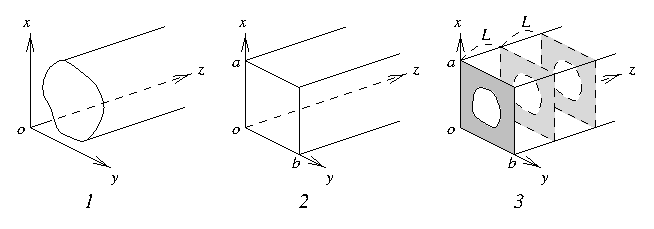
\includegraphics[clip]{1993phy2-1.eps}}
  \end{center}
\end{minipage}

但し、$\vec{D},\vec{E},\vec{B},\vec{H}$はそれぞれ電束密度、
電場、磁束密度、磁場(磁場の強さ)である。また$\rho,
\vec{j}$はそれぞれ電荷密度、電流密度である。\\

\end{question}
\begin{answer}{専攻 問題2}{}

\begin{subanswers}
\SubAnswer
  与えられた電場、磁場の式\eqhref{1}を
  $\vec{B}=\mu_{0}\vec{H},\;\vec{D}=\varepsilon_{0}\vec{E},\;\vec{j}=0$
  の条件のもと、Maxwell方程式\eqhref{M2}、\eqhref{M4}に代入すると、
%
  \[ \begin{array}{ll}
       \ds \Partial{E_{z}}{y}-ikE_{y}%
        = +i\mu_{0} \omega H_{x} \cdots (A) \qquad &
       \ds \Partial{H_{z}}{y}-ikH_{y}%
        = -i\varepsilon_{0} \omega E_{x} \cdots(C) \\[2mm]
       \ds ikE_{x}-\Partial{E_{z}}{x}%
        = +i\mu_{0} \omega H_{y} \cdots (B) \qquad &
       \ds ikH_{x}-\Partial{H_{z}}{x}%
        = -i\varepsilon_{0} \omega E_{y} \cdots (D) \\[2mm]
       \ds \Partial{E_{y}}{x}-\Partial{E_{x}}{y}%
        = +i\mu_{0} \omega H_{z} \cdots (E) \qquad &
       \ds \Partial{H_{y}}{x}-\Partial{H_{x}}{y}%
        = -i\varepsilon_{0} \omega E_{z} \cdots (F) \\
     \end{array} \]
%
  を得る。
%
  \[ \begin{array}{lcl}
       (A)\times \varepsilon_{0} \omega + (D)\times k    &より&
       \ds H_{x} = i\frac{k\Partial{H_{z}}{x}-\varepsilon_{0} \omega \Partial{E_{z}}{y}}{(\omega /c)^2-k^2} \\[3mm]
%
       (A)\times k + (D)\times \mu_{0} \omega            &より&
       \ds E_{y} = i\frac{k\Partial{E_{z}}{y}-\mu_{0}\omega \Partial{H_{z}}{x}}{(\omega /c)^2-k^2} \\[3mm]
%
       (B)\times (-\varepsilon_{0} \omega) + (C)\times k &より&
       \ds H_{y} = i\frac{k\Partial{H_{z}}{y}+\varepsilon_{0} \omega \Partial{E_{z}}{x}}{(\omega /c)^2-k^2}  \\[3mm]
%
       (B)\times k + (C)\times (-\mu_{0} \omega)         &より&
       \ds E_{x} = i\frac{k\Partial{E_{z}}{x}+\mu_{0} \omega 
\Partial{H_{z}}{y}}{(\omega /c)^2-k^2}
     \end{array} \]
%

\SubAnswer
  $(E),(F)$
   より、
%
  \[ H_{z} = \frac{1}{i\mu_{0} \omega} \left(
        \Partial{E_{y}}{x}-\Partial{E_{x}}{y} \right), \hspace{10mm} 
     E_{z} = -\frac{1}{i\varepsilon_{0} \omega} \left(
        \Partial{H_{y}}{x}-\Partial{H_{x}}{y} \right) \]
%
  これに{\bf 1}の結果を代入すると、
%
  \[ H_{z}=\frac{1}{(\omega /c)^{2}-k^{2}} \frac{1}{\mu_{0} \omega}
     \left[ k\Partial{}{x}\Partial{E_{z}}{y} -\mu_{0} \omega 
     \Partial{^{2}H_{z}}{x^{2}} - k\Partial{}{y}\Partial{E_{z}}{x} - 
     \mu_{0} \omega \Partial{^{2}H_{z}}{y^{2}}\right] \]
%
  整理して、
%
  \begin{equation}
    H_{z}=-\frac{1}{(\omega /c)^{2}-k^{2}}
    \left( \Partial{^{2}}{x^{2}}+\Partial{^{2}}{y^{2}} \right) H_{z}
    \eqname{3}
  \end{equation}
%
  同様にして
%
  \begin{equation}
    E_{z}=-\frac{1}{(\omega /c)^{2}-k^{2}}
    \left( \Partial{^{2}}{x^{2}}+\Partial{^{2}}{y^{2}} \right) E_{z}
    \eqname{4}
  \end{equation}
%
  上で得た方程式は$H_{z},E_{z}$が混ざり合っていない方程式であり、
  かつ、$H_{z}=0,E_{z}=0$は解であるのでTM波、TE波に分けて考えること
  ができる。


\newpage
\SubAnswer
  導体面上での電場と磁場の接続を考える。完全導体の場合、導体内の電場
  と磁場は0である。導体面と平行な成分を$E_{t},H_{t}$、垂直な成分を
  $E_{n},H_{n}$とする。すると
%
  \[ \left\{ \begin{array}{lcll}
       \Rot{\vec{E}} = -\Partial{\vec{B}}{t} &より&%
        E_{t}=0 & \\
       \Div{\vec{D}} = \rho &より&%
        E_{n}=\omega_{e}/{\varepsilon_{0}}&%
        \hspace{8mm} \omega_{e}:\;表面電荷密度 \\
       \Rot{\vec{H}} = \Partial{\vec{D}}{t}+\vec{j} &より&
        H_{t}=j_{\perp}&%
        \hspace{8mm} j_{\perp}:\;磁場と垂直な表面電流密度 \\
       \Div{\vec{B}} = 0 &より&
        H_{n}=0& \\
     \end{array} \right. \]
%
  となる。

  \leftline{\bf TM波の場合}
%
  $H_z=0$とおく。また、$x=0,y=0$での境界条件を考慮して$ E_z=C \sin{\xi x} \sin{\zeta y}$とおく。
  式\eqhref{4}に代入すると
%
  \[ \xi^{2}+\zeta^{2}=\left(\frac{\omega}{c} \right)^{2}-k^{2} \]
%
  境界で$E_z=0$なので
%
  \[ \begin{array}{lcl}
       \sin(\xi a)   = 0 &より&%
       \ds \xi=\frac{n\pi}{a},   \quad (n=1,2,3 \cdots) \\[3mm]
       \sin(\zeta b) = 0 &より&%
       \ds \zeta=\frac{m\pi}{b}, \quad (m=1,2,3 \cdots)
     \end{array} \]
%
  ここで$n=0$及び$m=0$は$E_z=0$を与えるので除く。よって
%
  \begin{equation}
    \left(\frac{\omega}{c} \right)^{2}-k^{2}%
      = \left(\frac{m^{2}}{b^{2}}+\frac{n^{2}}{a^{2}}\right)\pi^{2}
    \eqname{5}
  \end{equation}
%

  \leftline{\bf TE波の場合}
%
  $E_z=0,\;H_z=D \cos{\xi x} \cos{\zeta y}$とおく。
  式\eqhref{3}に代入すると
%
  \[ \xi^{2}+\zeta^{2}=\left(\frac{\omega}{c} \right)^{2}-k^{2} \]
%
  このとき
%
  \[ H_x=-i\frac{Dk\xi}{(\omega/c)^2-k^2}\sin{\xi x}\cos{\zeta y}%
     \hspace{10mm}%
     H_y=-i\frac{Dk\zeta}{(\omega/c)^2-k^2}\cos{\xi x}\sin{\zeta y}\]
%
  であり境界条件$x=0,a$ \ で$H_x=0$、$y=0,b$ \ で$H_y=0$なので
%
  \[ \begin{array}{lcl}
      \sin(\xi a)   = 0 &より&%
      \ds \xi=\frac{n\pi}{a}, \quad(n=0,1,2,3 \cdots) \\[3mm]
      \sin(\zeta b) = 0 &より&%
      \ds \zeta=\frac{m\pi}{b}, \quad(m=0,1,2,3 \cdots) \\
     \end{array} \]
%
  この場合も、
%
  \begin{equation}
    \left(\frac{\omega}{c} \right)^{2}-k^{2}%
    =\left( \frac{m^{2}}{b^{2}}+ \frac{n^{2}}{a^{2}} \right) \pi^{2}
    \eqname{6}
  \end{equation}
 
  式\eqhref{5}、\eqhref{6}をまとめて、$\omega$と$k$の関係は
%
  \begin{equation}
    \left( \frac{\omega}{c} \right)^{2}-k^{2}%
    = \left( \frac{m^{2}}{b^{2}}+ \frac{n^{2}}{a^{2}} \right) \pi^{2}%
    \hspace{8mm}%
    \left\{ \begin{array}{lc}%
      m,n = 1,2,3\cdots  ({\rm TM}) \\
      m,n = 0,1,2\cdots  ({\rm TE}) \qquad (m,n)=(0,0)\mbox{は除く。}\\
    \end{array} \right.
    \eqname{7}
  \end{equation}

  この両辺を$k$で偏微分して
%
  \[ 2\frac{\omega}{c^2}\Partial{\omega}{k}-2k=0 \hspace{8mm}%
     \frac{\omega}{k}\Partial{\omega}{k} = v_{p}\cdot v_{g} = c^2 \]


\SubAnswer
  式\eqhref{7}より、
%
  \[ \omega_{mn} = c \sqrt{k^{2}+\pi^{2}\left( \frac{m^2}{b^2}+
                   \frac{n^2}{a^2} \right)} \]
%
  $a>b$より最小の$\omega$は
%
  TM波の場合、$m=n=1$すなわち
  $\omega_{11}=c \sqrt{k^{2}+\pi^{2}%
  \left( \frac{1}{b^2}+\frac{1}{a^2} \right)}$
  であり、TE波の場合、$m=n=0$の時は$\eta^2=0$となり、
  これは$H_{x},E_{y},H_{y},E_{x}$の表式を見ると、
  分母が$0$となるので除く必要がある。よって$m=0,n=1$すなわち
  $\omega_{10}=c \sqrt{k^{2}+\pi^{2}\left( \frac{1}{a^2} \right)}$
  である。

  $\omega_{11}>\omega_{10}$より最小の$\omega$を与える電場、磁場は
  $\omega=\omega_{10}$のTE波である。この時、電場と磁場の値は\\
  $E_{z}=0,H_{z}=D\cos \left( \ds\frac{\pi}{a} x \right)$より
%
  \begin{eqnarray*}
   && E_{x}=0, \quad%
      E_{y}= i\frac{1}{(\omega/c)^2-k^2}\frac{\mu_{0}\omega \pi}{a}%
             D\sin \left( \frac{\pi}{a}x \right) \\
   && H_{x}=-i\frac{1}{(\omega/c)^2-k^2}\frac{k \pi}{a}%
             D\sin\left( \frac{\pi}{a}x \right), \quad%
      H_{y}=0
  \end{eqnarray*}
%
  となる。
 

\SubAnswer
  電場、磁場とも実数だから、
  $E(z)=\ds\frac{1}{2}\left( E_z\exp \{i(kz-\omega t)\} + 
  E_z^{*}\exp \{-i(kz-\omega t)\} \right)$と書ける。
  解は周期的になることが予想され、$E(z)$と$E(z+L)$は位相因子を除いて
  一致する。
%
  \[ E(z+L)=\ds\frac{1}{2}%
     \left( E_z\exp \{i(kz-\omega t)\}% 
     \exp(ikL) + E_z^{*}\exp \{-i(kz-\omega t)\} \exp (-ikL) \right) \]
%
  この式より$kL$は$2\pi$の整数倍になる必要があり、
  前問までは連続変数だった$k$が離散変数になることが求められる。
  つまり、$k=k_{l}=\ds\frac{2\pi l}{L}$($l$:整数)\\
%
  よって、分散関係も前問より
%
  \[ \omega_{nml}=c \sqrt{k_{l}^{2}+\pi^{2}%
     \left( \frac{m^2}{b^2}+\frac{n^2}{a^2} \right)}%
     =c\pi\sqrt{\frac{(2l)^2}{L^2}+\frac{m^2}{b^2}+\frac{n^2}{a^2}} \]
%
  と変更される。

\end{subanswers}
\end{answer}


\end{document}
